\section{Observational Data and Methods}
\label{sec:data-method}

We analyze public discussion archives from r/AmItheAsshole (AITA) to
examine how minority judgments are received (RQ1) and how they are
expressed and discussed (RQ2). We first define judgment alignment and
reception measures, then describe annotations of expressed certainty,
reply stance, and moral reasons. Figure~\ref{fig:study-overview}
illustrates how these measures and annotations relate to the discussion
structure. We also examine r/AITAH (AITAH) as a comparison community,
with additional results reported in the Appendix.

\begin{figure}[t]
  \centering
  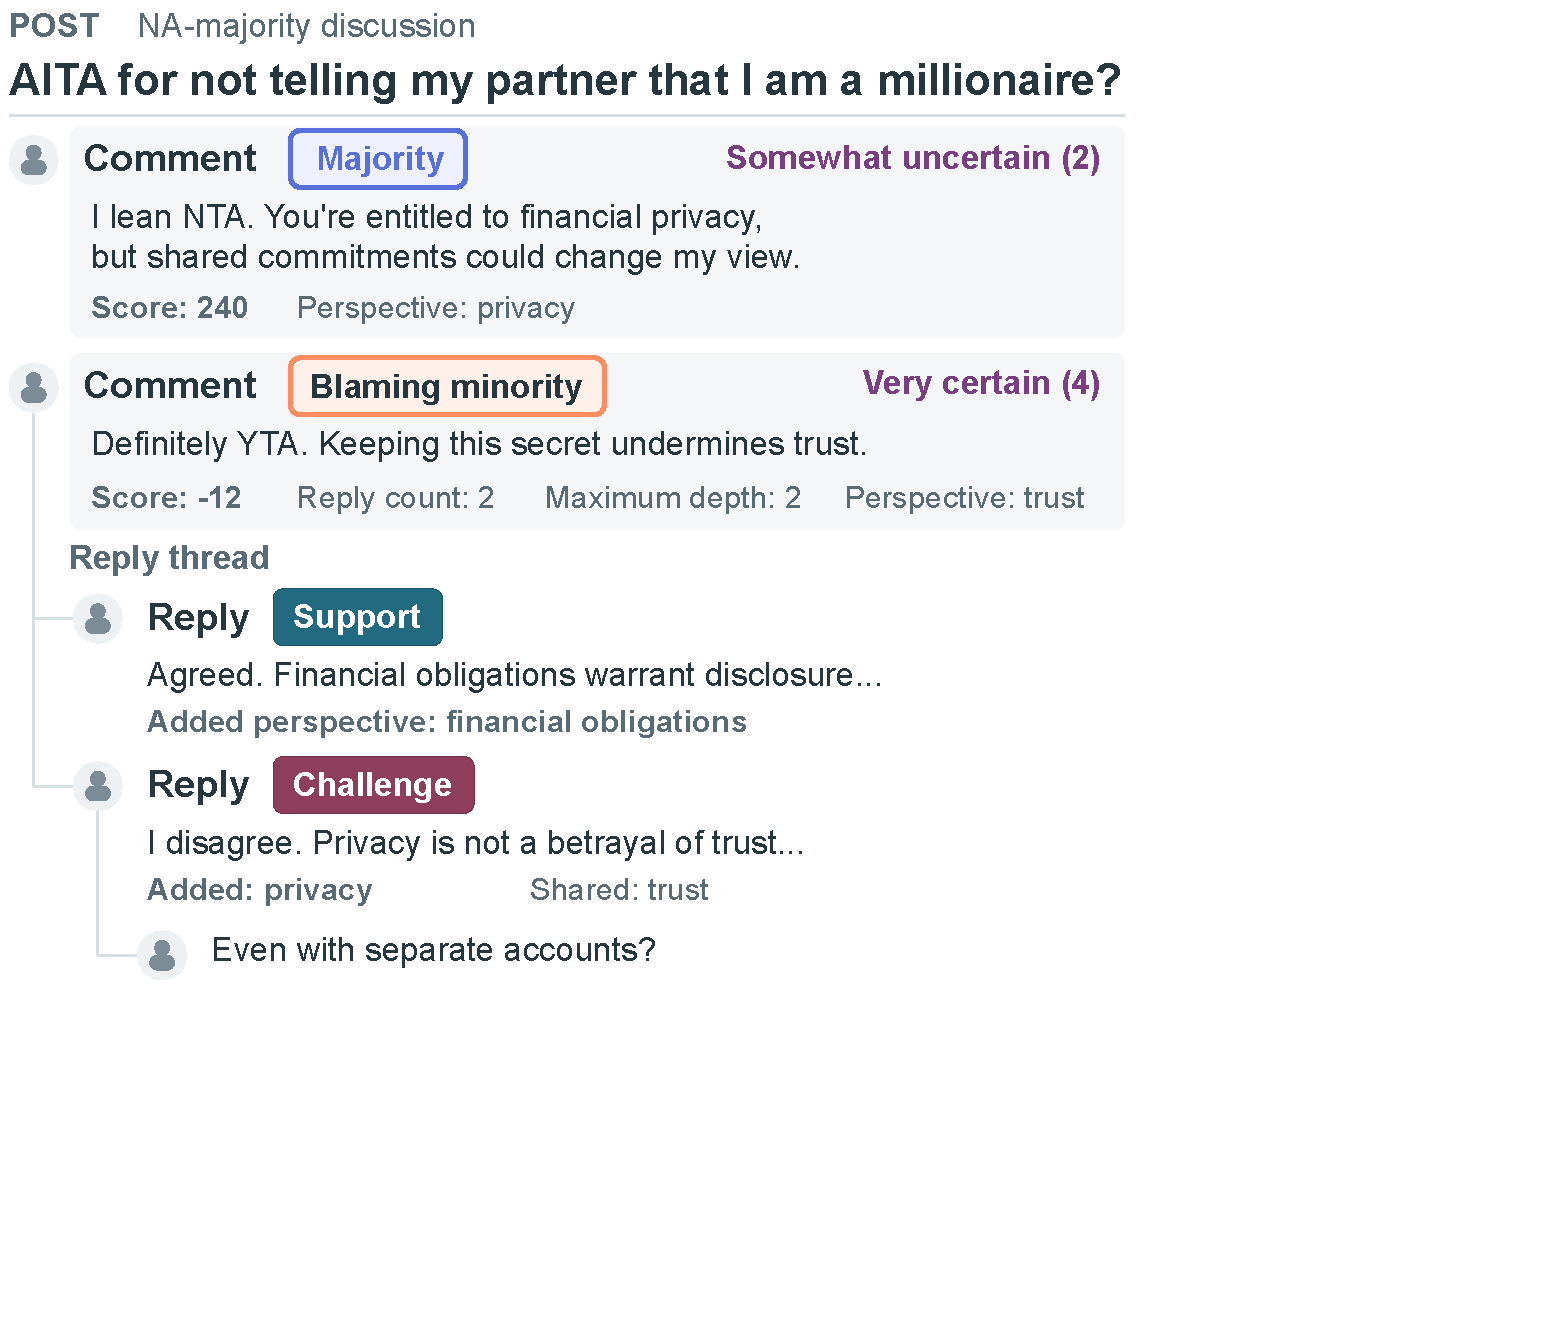
\includegraphics[width=\columnwidth]{figures/fig1_reddit.pdf}
  \caption{Illustrative AITA discussion linking structure, measures, and
  annotations. The blaming comment has two replies and maximum depth two.
  Added/shared perspectives are relative to the comment receiving each reply.
  The title is adapted; text, scores, and labels are schematic, not empirical results.}
  \label{fig:study-overview}
  \Description{An illustrative NA-majority discussion shows a somewhat
  uncertain majority comment and a very certain blaming minority comment.
  The latter has score minus twelve, two replies, and maximum reply depth two.
  A supporting reply adds financial obligations; a challenging reply adds
  privacy while sharing the comment's trust perspective. A further nested
  response illustrates depth two. All comments, scores, and labels are schematic.}
\end{figure}


\subsection{Discussion Data and Reception Measures}
\label{subsec:dataset}

A \emph{post} is its original poster's (OP's) account of an interpersonal
conflict. A \emph{comment} is a top-level response to the post;
a \emph{reply} responds directly to a comment. A \emph{reply thread}
includes replies to the comment and further nested responses.

\runinheading{Judgment categories.}
A \emph{judgment} assesses the OP's conduct. We group YTA
(``You're the Asshole'') and ESH (``Everyone Sucks Here'') as \emph{YA},
assigning fault to the OP; NTA (``Not the Asshole'') and NAH
(``No Assholes Here'') form \emph{NA}, assigning no fault to the OP.

\runinheading{Archive coverage and analytical samples.}
The public archives cover June 2013--December 2025 for AITA and
March 2021--December 2025 for AITAH. We exclude posts with empty or
removed bodies and use each comment's first recognized judgment
(matching rules in Appendix~\ref{sec:appendix-annotation-details};
variants in Appendix Table~\ref{tab:tags}). Judgment counts exclude
INFO (requests for information), comments without a recognized judgment,
and AutoModerator messages. Reception analyses use all available
judgment comments from posts with at least 200 judgments: 28,107 posts
in AITA and 8,217 in AITAH. Supplementary
Table~\ref{tab:analytical-samples} summarizes archive coverage and the
analytical samples; annotation-specific sampling procedures are described
in Section~\ref{subsec:method-annotation}.

\runinheading{\ai{Agreement and minority status.}}
\lx{A post’s \emph{dominant judgment} is whichever of YA or NA appears in more top-level comments.}
%The \emph{dominant judgment} is a post's more frequent judgement category, YA or NA.
\emph{Majority comments} match it; \emph{minority comments}, \lx{or \emph{dissent}}, oppose it.
%\ai{We use \emph{dissent} to denote judgments that differ from the post's dominant judgment.}
Comparisons requiring this distinction exclude exact ties.
\emph{High agreement} means at least 80\% favor one side;
\emph{low agreement} means each side accounts for 40--60\%.
\ai{Posts in which the dominant judgment accounts for more than 60\% but
less than 80\% of judgments are excluded from high-versus-low agreement
comparisons. We retain these posts when examining how reception varies
across the full range of agreement.}
\lxnote{need a pointer to where the additional results for the middle agreement lies}

\emph{Blaming dissent} assigns fault to an OP (\emph{YA}) whom the majority defends (\emph{NA});
\emph{defending dissent} defends an OP (\emph{NA}) whom the majority blames (\emph{YA}).
\ai{In Figure~\ref{fig:study-overview}, the post has an NA majority:
the NTA comment therefore represents the majority, while the YTA
comment represents blaming dissent.}

These directions concern different post sets.
\ai{We assign majority and minority status retrospectively during dataset
processing, using the final observed judgment distribution after the
discussions took place. These classifications remain fixed in temporal
analyses and do not reconstruct the distribution or comment order
readers encountered at the time. They reflect the observed comment
distribution rather than the community's official judgment. On Reddit,
comment visibility depends on sorting and ranking, including vote-based
ordering (see reception measures below). A prevailing judgment may be
easier to discern in high-agreement discussions; in low-agreement
discussions, readers may encounter either side first without perceiving
a clear majority. Dissent therefore describes a comment's relation to
the final observed majority, without assuming that its author recognized
or deliberately opposed that majority.}

\runinheading{Reception measures.}
\emph{Comment score} is the last recorded net score (upvotes minus downvotes).
\emph{Reply count} counts direct replies; \emph{maximum reply depth}
is the deepest level beneath a comment (zero without replies,
one for replies without further nesting). These measures use stored judgment labels
and reply structure\ai{; the text and author exclusions used for
annotation do not apply to reception measures.}

\ai{The minority comment in Figure~\ref{fig:study-overview} has a score
of $-12$, two direct replies, and a maximum reply depth of two. The nested
response contributes to depth but is not counted as a direct reply to
the top-level comment.}

We average comments within each post and judgment group, then weight
posts equally. Empty groups are omitted, not assigned zero; missing
scores affect only score averages. Contributing post sets may therefore
differ between groups. Outcomes use all available observations rather
than a uniform follow-up period. Arrival-time profiles group comments by
their posting hour during the first 24 hours; contributing post sets can
vary by hour. Appendix~\ref{sec:appendix-annotation-details} summarizes
aggregation and inference.

\subsection{\ai{Annotation of Comments and Replies}}
\label{subsec:method-annotation}

\ai{We annotate how firmly comments express their judgments, how direct
replies respond to those judgments, and whether replies introduce
additional moral reasons. Figure~\ref{fig:study-overview} distinguishes
certainty at the comment level from reply stance and the addition of
reasons relative to a parent comment.}

\runinheading{\ai{Expressed certainty.}}
To compare how firmly majority and minority comments express their judgments,
we use comment-level certainty annotations from sampled high- and
low-agreement posts. The scale captures
expressed language, not private confidence: very uncertain (1), somewhat
uncertain (2), somewhat certain (3), and very certain (4). The same
criteria apply across judgments.

We compare certainty distributions and the proportion at level 4 between
blaming and defending dissent over the full observed period, weighting
posts equally. These estimates describe the annotated sample, not
community-wide certainty.

To compare expression as discussions progress, we divide the first
24 hours of judgment comments in high-agreement AITA posts into ten
chronological stages containing approximately equal numbers of comments.
We compare majority, blaming minority, and defending
minority comments using equal post weights. For each group, we retain a
fixed set of posts with at least one comment from that group with a valid
certainty annotation in every stage, keeping post composition constant
across stages. Post fixed-effects regressions estimate linear changes
across the sequence. These analyses describe successive comments in the
selected discussions, not changes within individuals.
Estimation and sensitivity checks are summarized in
Appendices~\ref{sec:appendix-annotation-details} and~\ref{sec:appendix-evidence}.

\runinheading{Reply stance.}
Whereas certainty compares how firmly judgments are expressed, reply
stance captures how others respond. Drawing on prior work~\citep{andreas2012annotating}, we classify replies (towards their top-level comments) into four response categories:
\emph{support} (endorsing the parent's position), \emph{challenge}
(disputing it), \emph{information-seeking} (requesting clarification), and
\emph{other}.

We sample three stratified sets of 16,000 top-level comment--direct reply
pairs from high-agreement posts while excluding pairs involving OPs, who are parties to the conflict and may reply to explain or defend their conduct~\citep{giorgi2023author}.
Given the post as context, an LLM classifies each reply's stance toward its parent comment.

\begin{comment}
We annotate reply stance to distinguish endorsement from opposition within
the engagement captured by reply counts. We use three samples of 16,000
comment--reply pairs each from high-agreement posts, excluding OP
participation. Unlike other commenters, OPs are
parties to the conflict and may use replies to explain or defend their own
conduct. Excluding their participation focuses the analysis on how other
community members respond to judgments.
Given the post as context, DeepSeek labels each reply's stance toward its comment, with human review of 100 development-set pairs. Labels distinguish \emph{support}, which endorses the comment's position; \emph{challenge}, which disputes it;
\emph{information-seeking}, which requests clarification; and \emph{other},
which covers remaining functions.
Challenge denotes disagreement, not necessarily personal attack. Proportions weight eligible comment--reply pairs equally and describe reply composition, not all comments.
\end{comment}

\runinheading{Additional moral reasons.}
We also examine whether replies introduce moral reasons absent from their parent comments.
We analyze 7,023 eligible pairs from 100 high-agreement AITA posts, alongside their reply stances.
To identify the moral reasons in these comments, we use a two-stage LLM-based procedure inspired by inductive category formation~\citep{mayring2014qualitative}.
First, we construct a taxonomy of moral reasons for each post through iterative refinement.
We then use the resulting categories to label top-level comments and their direct replies, allowing multiple labels for each.
A reply is coded as adding a moral reason category if it receives a label absent from its parent comment.
For example, in Figure~\ref{fig:study-overview}, the supporting and challenging replies add financial obligations and privacy, respectively, beyond the parent's concern with trust.
More details about the annotation process are provided in Appendix~\ref{sec:appendix-annotation-details}.

\begin{comment}
\ai{In Figure~\ref{fig:study-overview}, the supporting reply adds financial obligations, while the challenging reply adds privacy beyond the
parent's concern with trust. Privacy counts as an addition even though
it appears in another comment: addition is assessed relative to the
parent, not the discussion as a whole.}
\end{comment}

Within each post, parent group, and reply stance, proportions include all eligible replies, including those assigned no
category; empty cells are omitted. We average these proportions across
posts with equal weight and estimate $95\%$ percentile CIs from 20,000
joint whole-post bootstrap resamples.
For exploratory comparisons of the displayed means, we use two-sided,
centered studentized bootstrap tests with 99,999 joint whole-post
resamples, preserving dependence between cells from the same post.
We test all three pairwise parent-group contrasts within each of the
three reply subsets (all, support, and challenge), plus challenge versus
support within each parent group. Holm adjustment covers these 12
comparisons as one family. Contrasts compare marginal post-equal means
using each cell's contributing posts, rather than restricting both cells
to their shared posts. These tests treat model-assigned labels as fixed;
they do not account for classification uncertainty or omitted category
assignments.
